\documentclass[12pt]{article}

\usepackage{amsmath,amssymb,amsthm}
\usepackage{geometry}
\usepackage{microtype}
\usepackage{setspace}
\usepackage{fontspec}
\usepackage{booktabs}
\usepackage{array}
\usepackage{listings}
\usepackage{xcolor}
\usepackage{hyperref}
\usepackage[nameinlink]{cleveref}
\usepackage{tikz}
\usetikzlibrary{
  arrows.meta,
  positioning,
  calc,
  decorations.pathmorphing,
  decorations.markings,
  shapes.geometric,
  shapes.multipart,
  fit,
  backgrounds,
  patterns,
  hobby,
}

\geometry{margin=1.3in}
\setmainfont{Linux Libertine O}
\setmonofont{Linux Libertine Mono O}
\onehalfspacing

%% IPA name: slashes in monospace, IPA characters in main serif font
%% (Linux Libertine Mono lacks ː and ɛ; Linux Libertine O has both)
\newcommand{\ambibf}{%
  \texttt{/}\textnormal{æmbiːɛf}\texttt{/}%
}

\definecolor{codebg}{gray}{0.96}
\definecolor{codecomment}{gray}{0.45}
\definecolor{codestring}{RGB}{0,100,0}
\definecolor{codekeyword}{RGB}{0,0,160}
\definecolor{linkblue}{RGB}{30,60,140}

\lstset{
  language=Python,
  backgroundcolor=\color{codebg},
  basicstyle=\small\ttfamily,
  keywordstyle=\color{codekeyword},
  stringstyle=\color{codestring},
  commentstyle=\color{codecomment}\itshape,
  breaklines=true,
  frame=single,
  framesep=4pt,
  xleftmargin=6pt,
  xrightmargin=6pt,
  showstringspaces=false,
  tabsize=4,
}

\newtheorem{theorem}{Theorem}[section]
\newtheorem{lemma}[theorem]{Lemma}
\newtheorem{definition}[theorem]{Definition}

\hypersetup{
  colorlinks=true,
  linkcolor=linkblue,
  urlcolor=linkblue,
  citecolor=linkblue,
}

\title{{\large\bfseries Globally Persistent Recomposable Thought}\\[4pt]
{\normalsize GitHub, the Intelligence Explosion, and\\
the Admissibility Geometry of Collective Cognition}}
\author{Flyxion}
\date{\today}

\begin{document}
\maketitle

\begin{abstract}
The conventional narrative attributes the current acceleration in technological
capability to the emergence of generative artificial intelligence. This essay
argues that this attribution is substantially mislocated. The more fundamental
cause is a structural transformation in the organization of human technical
cognition that preceded large language models by nearly two decades: the
creation, through GitHub and adjacent open-source infrastructure, of a globally
persistent, recursively recomposable substrate for executable thought. Generative
AI functions as a compression interface and navigational accelerant over that
substrate, not as its source. We develop this argument in five stages: first, as
a historical and infrastructural claim about the bottlenecks that GitHub
dissolved; second, as an epistemic economy argument about the incentive
structures GitHub created across academia, industry, and independent research;
third, through a concrete worked example in which Spherepop semantics are
implemented over the probabilistic substrate language \ambibf{},
demonstrating the three-tier taxonomy of admissible, boundary, and inert
repository contributions; fourth, as a connection to the Quantum SpherePop
field-theoretic framework, in which developmental geometry is interpreted as
a semantic quantization sequence and repository replay is formalized as
coarse-grained semantic reconstruction; and fifth, as a connection to the RSVP
admissibility framework, in which the GitHub substrate is understood as a
planetary-scale coherence field whose dynamics are governed by the same
lamphron--lamphrodyne duality that governs physical structure formation.
Mathematical appendices formalize the stochastic tape geometry, bubble energy,
mortality functional, stabilization operators, and attractor semantics of the
worked example.
\end{abstract}

\tableofcontents
\clearpage
%% figures.tex
%% All TikZ figures for "Globally Persistent Recomposable Thought"
%% Black and white. TikZ libraries loaded in main preamble.

%% ─────────────────────────────────────────────────────────────────────────────
%% FIGURE 1: Substrate vs Accelerant architecture
%% ─────────────────────────────────────────────────────────────────────────────
\begin{figure}[htbp]
\centering
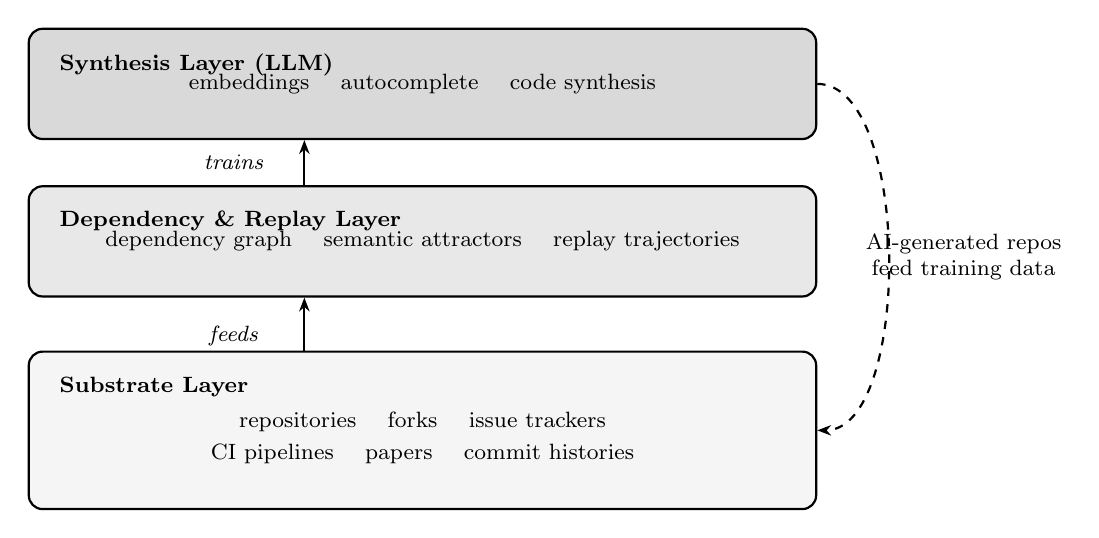
\begin{tikzpicture}[
  font=\small,
  every node/.style={align=center},
  layer/.style={draw=black, thick, rounded corners=5pt, minimum width=10cm},
  sublabel/.style={font=\footnotesize},
  arrow/.style={-{Stealth[length=5pt]}, thick},
  recurse/.style={-{Stealth[length=5pt]}, thick, dashed},
]

\node[layer, fill=gray!8, minimum height=2.0cm] (substrate) at (0,0) {};
\node[anchor=north west, font=\footnotesize\bfseries]
  at (substrate.north west) [xshift=8pt, yshift=-6pt] {Substrate Layer};
\node[sublabel] at (0,-0.1)
  {repositories \quad forks \quad issue trackers\\[2pt]
   CI pipelines \quad papers \quad commit histories};

\node[layer, fill=gray!18, minimum height=1.4cm] (graph) at (0, 2.4) {};
\node[anchor=north west, font=\footnotesize\bfseries]
  at (graph.north west) [xshift=8pt, yshift=-6pt]
  {Dependency \& Replay Layer};
\node[sublabel] at (0,2.4)
  {dependency graph \quad semantic attractors \quad replay trajectories};

\node[layer, fill=gray!30, minimum height=1.4cm] (model) at (0, 4.4) {};
\node[anchor=north west, font=\footnotesize\bfseries]
  at (model.north west) [xshift=8pt, yshift=-6pt] {Synthesis Layer (LLM)};
\node[sublabel] at (0,4.4)
  {embeddings \quad autocomplete \quad code synthesis};

\draw[arrow] ([xshift=-1.5cm]substrate.north) -- ([xshift=-1.5cm]graph.south);
\draw[arrow] ([xshift=-1.5cm]graph.north)     -- ([xshift=-1.5cm]model.south);
\node[font=\footnotesize\itshape] at (-2.4, 1.2) {feeds};
\node[font=\footnotesize\itshape] at (-2.4, 3.4) {trains};

%% Recursive loop — on right, tight to box
\draw[recurse]
  (model.east) .. controls +(1.2,0) and +(1.2,0) .. (substrate.east);
\node[font=\footnotesize, right=14pt] at (model.east |- {(0,2.2)})
  {AI-generated repos\\feed training data};

\end{tikzpicture}
\caption{The substrate--accelerant architecture. The LLM synthesis layer sits
\emph{inside} a larger recursion loop: models generate repositories that feed
future training. The substrate layer preceded the synthesis layer by over a
decade.}
\label{fig:substrate}
\end{figure}

%% ─────────────────────────────────────────────────────────────────────────────
%% FIGURE 2: Three tiers of admissibility (geometric)
%% ─────────────────────────────────────────────────────────────────────────────
\begin{figure}[htbp]
\centering
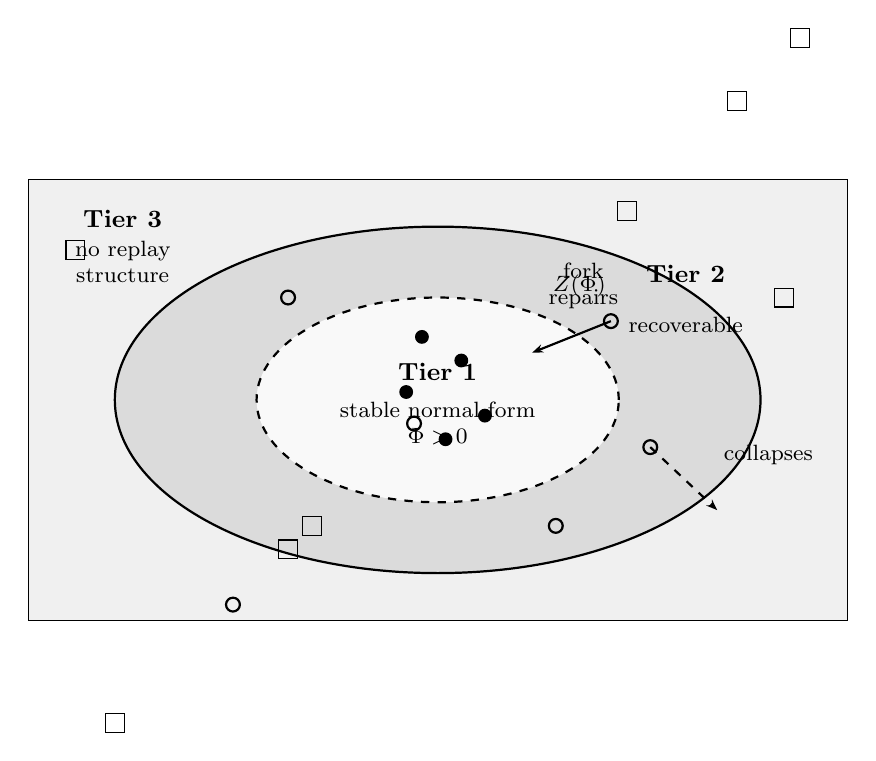
\begin{tikzpicture}[
  font=\small,
  every node/.style={align=center},
]

\fill[gray!12] (-5.2,-2.8) rectangle (5.2,2.8);
\draw[black] (-5.2,-2.8) rectangle (5.2,2.8);

\fill[gray!28] (0,0) ellipse (4.1cm and 2.2cm);
\draw[black, thick] (0,0) ellipse (4.1cm and 2.2cm);

\fill[gray!5] (0,0) ellipse (2.3cm and 1.3cm);
\draw[black, thick, dashed] (0,0) ellipse (2.3cm and 1.3cm);

\node[font=\footnotesize] at (1.8, 1.45) {$Z(\Phi)$};

\node[font=\small\bfseries] at (0, 0.35) {Tier 1};
\node[font=\footnotesize] at (0,-0.3) {stable normal form\\$\Phi>0$};

\node[font=\small\bfseries] at (3.15, 1.6) {Tier 2};
\node[font=\footnotesize] at (3.15, 0.95) {recoverable};

\node[font=\small\bfseries] at (-4.0, 2.3) {Tier 3};
\node[font=\footnotesize] at (-4.0, 1.75) {no replay\\structure};

\foreach \x/\y in {0.3/0.5,-0.4/0.1,0.1/-0.5,-0.2/0.8,0.6/-0.2}{
  \fill[black] (\x,\y) circle (2.5pt);
}
\foreach \x/\y in {2.2/1.0,-1.9/1.3,2.7/-0.6,-2.6,-0.3,1.5/-1.6}{
  \draw[black, thick] (\x,\y) circle (2.5pt);
}
\foreach \x/\y in {4.4/1.3,-4.6/1.9,4.6,-1.6,-4.1,-1.9,3.8,2.4}{
  \draw[black] (\x-0.12,\y-0.12) rectangle (\x+0.12,\y+0.12);
}

\draw[-{Stealth[length=4pt]}, thick] (2.2,1.0) -- (1.2,0.6);
\node[font=\footnotesize] at (1.85, 1.45) {fork\\repairs};

\draw[-{Stealth[length=4pt]}, thick, dashed] (2.7,-0.6) -- (3.55,-1.4);
\node[font=\footnotesize] at (4.2,-0.7) {collapses};

\end{tikzpicture}
\caption{The three tiers of admissibility. Tier~1 (inner, white): stable
$\Phi>0$, robust contribution. Tier~2 (middle gray annulus): near $Z(\Phi)$,
recoverable via forking. Tier~3 (outer, darker): no replay structure,
outside the admissibility manifold.}
\label{fig:admissibility}
\end{figure}

%% ─────────────────────────────────────────────────────────────────────────────
%% FIGURE 3: Replay geometry
%% ─────────────────────────────────────────────────────────────────────────────
\begin{figure}[p]
\centering
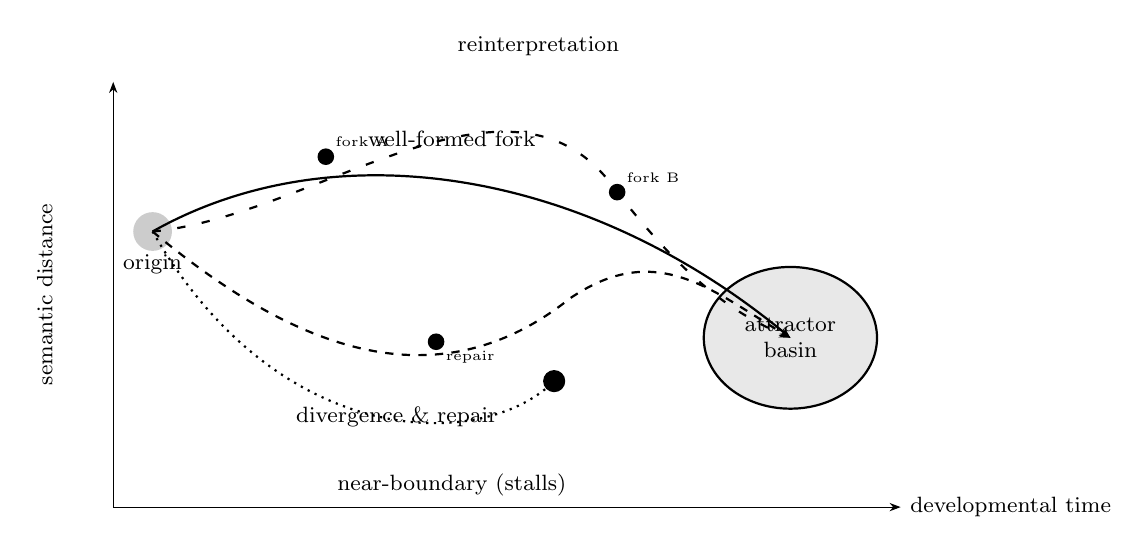
\begin{tikzpicture}[
  font=\small,
  every node/.style={align=center},
]

\fill[gray!18] (7.8,-1.35) ellipse (1.1cm and 0.9cm);
\draw[black, thick] (7.8,-1.35) ellipse (1.1cm and 0.9cm);
\node[font=\footnotesize] at (7.8,-1.35) {attractor\\basin};

\fill[gray!40] (-0.3,0) circle (7pt);
\node[font=\footnotesize, below=5pt] at (-0.3,0) {origin};

\draw[black, thick, -{Stealth[length=4pt]}]
  (-0.3,0) .. controls (2,1.3) and (5.2,0.8) .. (7.8,-1.35);
\node[font=\footnotesize, above] at (3.5, 0.95) {well-formed fork};

\draw[black, thick, dashed, -{Stealth[length=4pt]}]
  (-0.3,0) .. controls (1.5,-1.5) and (3.3,-2.2) ..
  (5.0,-0.85) .. controls (6.1,-0.1) and (6.8,-0.75) .. (7.8,-1.35);
\node[font=\footnotesize] at (2.8,-2.35) {divergence \& repair};

\draw[black, thick, loosely dashed, -{Stealth[length=4pt]}]
  (-0.3,0) .. controls (1.8,0.2) and (4.3,2.4) ..
  (5.6,0.5) .. controls (6.5,-0.65) and (7.1,-1.05) .. (7.8,-1.35);
\node[font=\footnotesize] at (4.6, 2.35) {reinterpretation};

\draw[black, thick, dotted]
  (-0.3,0) .. controls (1.3,-2.8) and (3.9,-2.8) .. (4.8,-1.9);
\fill[black] (4.8,-1.9) circle (4pt);
\node[font=\footnotesize, below] at (3.5,-2.95) {near-boundary (stalls)};

\fill[black] (1.9,0.95) circle (3pt);
\node[font=\tiny, above right] at (1.9,0.95) {fork A};
\fill[black] (3.3,-1.4) circle (3pt);
\node[font=\tiny, below right] at (3.3,-1.4) {repair};
\fill[black] (5.6,0.5) circle (3pt);
\node[font=\tiny, above right] at (5.6,0.5) {fork B};

\draw[-{Stealth[length=4pt]}] (-0.8,-3.5) -- (9.2,-3.5);
\node[font=\footnotesize, right] at (9.2,-3.5) {developmental time};
\draw[-{Stealth[length=4pt]}] (-0.8,-3.5) -- (-0.8,1.9);
\node[font=\footnotesize, rotate=90, above] at (-1.45,-0.8) {semantic distance};

\end{tikzpicture}
\caption{Repository replay as braided attractor trajectories. Forks, repairs,
and reinterpretations converge on the attractor basin despite local divergence.
Near-boundary trajectories may stall. The basin is defined by convergence of
the replay distribution $\sigma_n \sim \mathbb{P}_n$.}
\label{fig:replay}
\end{figure}

%% ─────────────────────────────────────────────────────────────────────────────
%% FIGURE 4: Lamphron–lamphrodyne dual cycle
%% ─────────────────────────────────────────────────────────────────────────────
\begin{figure}[p]
\centering
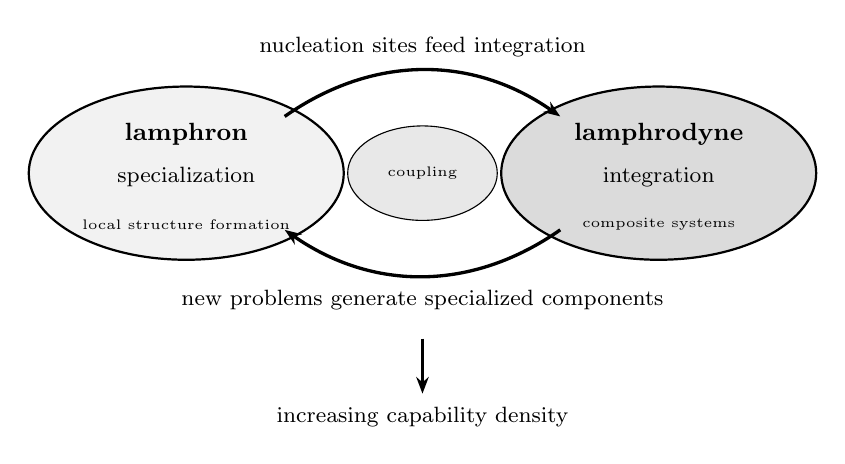
\begin{tikzpicture}[
  font=\small,
  every node/.style={align=center},
  vortex/.style={draw=black, thick, ellipse,
                 minimum width=4.0cm, minimum height=2.2cm},
  arrow/.style={-{Stealth[length=6pt]}, very thick},
]

\node[vortex, fill=gray!10] (L) at (-3.0,0) {};
\node[font=\small\bfseries] at (-3.0, 0.5) {lamphron};
\node[font=\footnotesize] at (-3.0,-0.05) {specialization};
\node[font=\tiny] at (-3.0,-0.65) {local structure formation};

\node[vortex, fill=gray!28] (R) at (3.0,0) {};
\node[font=\small\bfseries] at (3.0, 0.5) {lamphrodyne};
\node[font=\footnotesize] at (3.0,-0.05) {integration};
\node[font=\tiny] at (3.0,-0.65) {composite systems};

\fill[gray!18] (0,0) ellipse (0.95cm and 0.6cm);
\draw[black] (0,0) ellipse (0.95cm and 0.6cm);
\node[font=\tiny] at (0,0) {coupling};

\draw[arrow, bend left=35]
  (-1.75,0.72) to
  node[above, font=\footnotesize, yshift=1pt]
  {nucleation sites feed integration}
  (1.75,0.72);

\draw[arrow, bend left=35]
  (1.75,-0.72) to
  node[below, font=\footnotesize, yshift=-1pt]
  {new problems generate specialized components}
  (-1.75,-0.72);

\draw[arrow] (0,-2.1) -- (0,-2.8);
\node[font=\footnotesize] at (0,-3.1) {increasing capability density};

\end{tikzpicture}
\caption{The lamphron--lamphrodyne dual cycle. Lamphron (compact, specialized)
repositories create conditions for lamphrodyne integration (composite systems).
Integration generates new problems that spawn new specialized repositories,
closing the recursive loop.}
\label{fig:lamphron}
\end{figure}

%% ─────────────────────────────────────────────────────────────────────────────
%% FIGURE 5: Semantic quantization sequence
%% ─────────────────────────────────────────────────────────────────────────────
\begin{figure}[p]
\centering
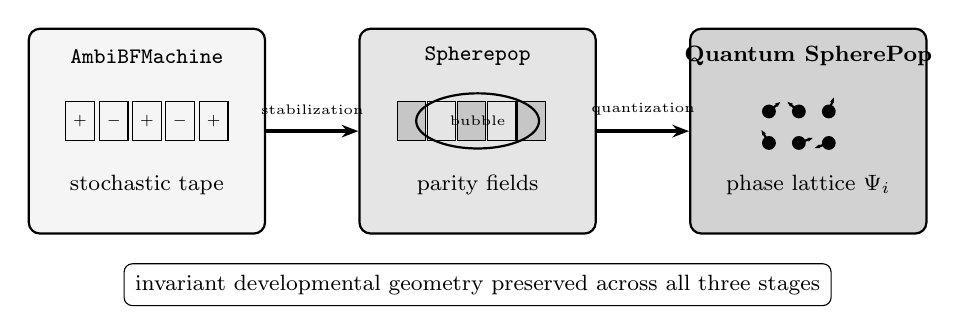
\begin{tikzpicture}[
  font=\small,
  every node/.style={align=center},
  stage/.style={draw=black, thick, rounded corners=4pt,
                minimum width=3.0cm, minimum height=2.6cm},
  arrow/.style={-{Stealth[length=6pt]}, very thick},
]

\node[stage, fill=gray!8] (S1) at (0,0) {};
\node[font=\footnotesize\bfseries] at (0,0.95) {\texttt{AmbiBFMachine}};
\foreach \i/\v in {-0.85/{$+$},-0.42/{$-$},0/{$+$},0.42/{$-$},0.85/{$+$}}{
  \draw[black] (\i-0.18,-0.12) rectangle (\i+0.18,0.38);
  \node[font=\tiny] at (\i,0.13) {\v};
}
\node[font=\footnotesize] at (0,-0.68) {stochastic tape};

\node[stage, fill=gray!20] (S2) at (4.2,0) {};
\node[font=\footnotesize\bfseries] at (4.2,0.95) {\texttt{Spherepop}};
\foreach \i in {-0.84,-0.08,0.68}{
  \fill[gray!45] (\i+4.2-0.18,-0.12) rectangle (\i+4.2+0.18,0.38);
  \draw[black] (\i+4.2-0.18,-0.12) rectangle (\i+4.2+0.18,0.38);
}
\foreach \i in {-0.46,0.30}{
  \draw[black] (\i+4.2-0.18,-0.12) rectangle (\i+4.2+0.18,0.38);
}
\draw[black, thick] (4.2,0.13) ellipse (0.78cm and 0.35cm);
\node[font=\tiny] at (4.2,0.13) {bubble};
\node[font=\footnotesize] at (4.2,-0.68) {parity fields};

\node[stage, fill=gray!35] (S3) at (8.4,0) {};
\node[font=\footnotesize\bfseries] at (8.4,0.95) {Quantum SpherePop};
\foreach \x/\y/\th in
  {-0.5/0.25/40,-0.12/0.25/140,0.26/0.25/70,
   -0.5/-0.15/120,-0.12/-0.15/20,0.26/-0.15/200}{
  \fill[black] (\x+8.4,\y) circle (2.5pt);
  \draw[-{Stealth[length=2pt]}, black, thick]
    (\x+8.4,\y) -- +({cos(\th)*0.19},{sin(\th)*0.19});
}
\node[font=\footnotesize] at (8.4,-0.68) {phase lattice $\Psi_i$};

\draw[arrow] (S1.east) -- node[above,font=\tiny,yshift=2pt]
  {stabilization} (S2.west);
\draw[arrow] (S2.east) -- node[above,font=\tiny,yshift=2pt]
  {quantization} (S3.west);

\node[font=\footnotesize, draw=black, rounded corners=3pt,
      inner sep=4pt, fill=white]
  at (4.2,-1.95)
  {invariant developmental geometry preserved across all three stages};

\end{tikzpicture}
\caption{The semantic quantization sequence. \texttt{AmbiBFMachine}: raw
stochastic tape. \texttt{Spherepop}: parity-preserving metastable bubbles.
Quantum SpherePop: coupled phase lattice $\Psi_i = r_i e^{i\theta_i}$.
Each stage preserves invariant developmental geometry while increasing
representational richness.}
\label{fig:quantization}
\end{figure}

%% ─────────────────────────────────────────────────────────────────────────────
%% FIGURE 6: GitHub as externalized working memory
%% ─────────────────────────────────────────────────────────────────────────────
\begin{figure}[p]
\centering
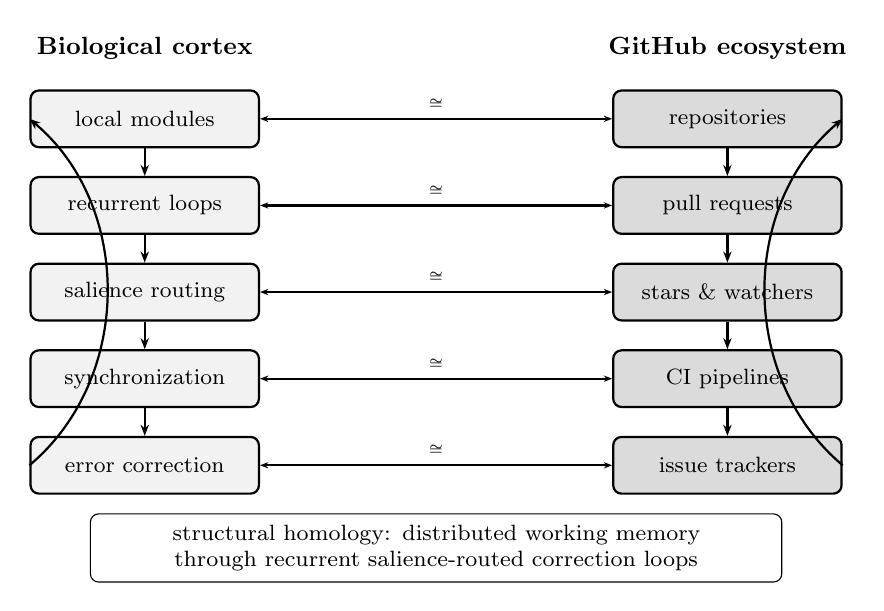
\begin{tikzpicture}[
  font=\small,
  every node/.style={align=center},
  block/.style={draw=black, thick, rounded corners=3pt,
                minimum width=2.9cm, minimum height=0.72cm, font=\footnotesize},
  arrow/.style={-{Stealth[length=4pt]}, thick},
  hlabel/.style={font=\small\bfseries},
]

\node[hlabel] at (-3.7,3.1) {Biological cortex};
\node[hlabel] at (3.7,3.1)  {GitHub ecosystem};

\node[block,fill=gray!10]  (bmod)   at (-3.7,2.2) {local modules};
\node[block,fill=gray!10]  (brecur) at (-3.7,1.1) {recurrent loops};
\node[block,fill=gray!10]  (bsal)   at (-3.7,0.0) {salience routing};
\node[block,fill=gray!10]  (bsync)  at (-3.7,-1.1) {synchronization};
\node[block,fill=gray!10]  (berr)   at (-3.7,-2.2) {error correction};

\draw[arrow] (bmod)--(brecur); \draw[arrow] (brecur)--(bsal);
\draw[arrow] (bsal)--(bsync); \draw[arrow] (bsync)--(berr);
\draw[arrow, bend right=50] (berr.west) to (bmod.west);

\node[block,fill=gray!28] (grepo) at (3.7,2.2)  {repositories};
\node[block,fill=gray!28] (gpr)   at (3.7,1.1)  {pull requests};
\node[block,fill=gray!28] (gstar) at (3.7,0.0)  {stars \& watchers};
\node[block,fill=gray!28] (gci)   at (3.7,-1.1) {CI pipelines};
\node[block,fill=gray!28] (giss)  at (3.7,-2.2) {issue trackers};

\draw[arrow] (grepo)--(gpr); \draw[arrow] (gpr)--(gstar);
\draw[arrow] (gstar)--(gci); \draw[arrow] (gci)--(giss);
\draw[arrow, bend left=50] (giss.east) to (grepo.east);

\foreach \l/\r in {bmod/grepo,brecur/gpr,bsal/gstar,bsync/gci,berr/giss}{
  \draw[{Stealth[length=3pt]}-{Stealth[length=3pt]}, thick]
    (\l.east) -- node[font=\tiny,above] {$\cong$} (\r.west);
}

\node[font=\footnotesize, draw=black, rounded corners=3pt,
      inner sep=4pt, fill=white, text width=8.5cm]
  at (0,-3.25)
  {structural homology: distributed working memory through
   recurrent salience-routed correction loops};

\end{tikzpicture}
\caption{Structural homology between the biological cortex and the GitHub
ecosystem. Both implement distributed working memory through analogous
functional layers. The homology is functional and architectural.}
\label{fig:cortex}
\end{figure}

%% ─────────────────────────────────────────────────────────────────────────────
%% FIGURE 7 (Appendix): Parity-preserving bubble region
%% ─────────────────────────────────────────────────────────────────────────────
\begin{figure}[htbp]
\centering
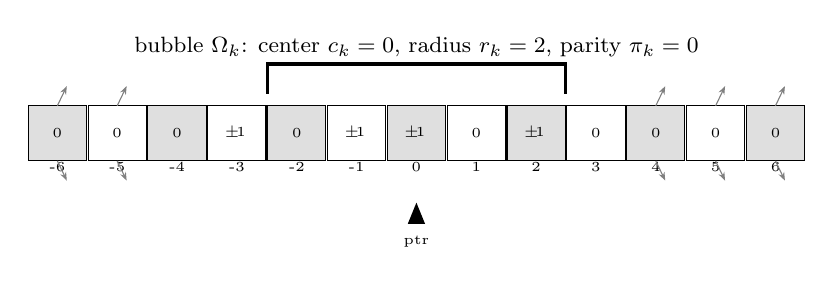
\begin{tikzpicture}[
  font=\small,
  every node/.style={align=center},
  cell/.style={draw=black, minimum width=0.74cm, minimum height=0.7cm,
               font=\footnotesize},
]

\foreach \i in {-6,...,6}{
  \pgfmathparse{mod(\i,2)==0 ? "gray!25" : "white"}
  \edef\fillcol{\pgfmathresult}
  \node[cell, fill=\fillcol] (C\i) at (\i*0.76,0) {};
  \node[font=\tiny, below=7pt] at (\i*0.76,0) {\i};
}

\foreach \i/\v in
  {-6/0,-5/0,-4/0,-3/{$\!\pm\!1$},-2/0,-1/{$\!\pm\!1$},
   0/{$\!\pm\!1$},1/0,2/{$\!\pm\!1$},3/0,4/0,5/0,6/0}{
  \node[font=\tiny] at (\i*0.76,0) {\v};
}

\draw[black, very thick]
  (-2*0.76-0.37,0.5) -- (-2*0.76-0.37,0.88)
  -- (2*0.76+0.37,0.88) -- (2*0.76+0.37,0.5);
\node[font=\footnotesize] at (0,1.1)
  {bubble $\Omega_k$: center $c_k=0$, radius $r_k=2$, parity $\pi_k=0$};

\foreach \i in {-6,-5,4,5,6}{
  \draw[-{Stealth[length=3pt]},black!50]
    (\i*0.76,0.35) -- +({0.12},{0.25});
  \draw[-{Stealth[length=3pt]},black!50]
    (\i*0.76,-0.35) -- +({0.12},{-0.25});
}

\fill[black] (0,-0.88) -- (-0.11,-1.15) -- (0.11,-1.15) -- cycle;
\node[font=\tiny,below=1pt] at (0,-1.15) {ptr};

\end{tikzpicture}
\caption{Parity-preserving bubble region on the \ambibf{} tape. Gray cells
(even index) form the bubble support $\Omega_k$. Drift arrows on exterior
cells illustrate stochastic noise the bubble must survive.}
\label{fig:bubble}
\end{figure}

%% ─────────────────────────────────────────────────────────────────────────────
%% FIGURE 8 (Appendix): Semantic mortality and stabilization
%% ─────────────────────────────────────────────────────────────────────────────
\begin{figure}[htbp]
\centering
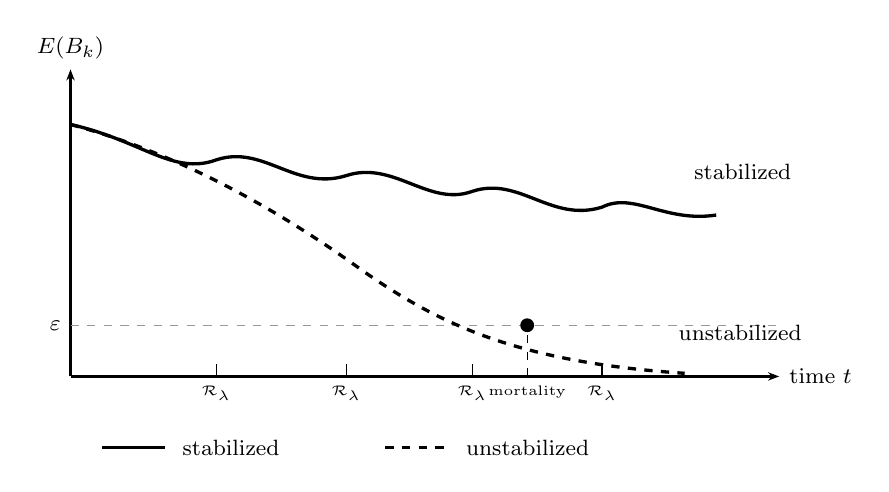
\begin{tikzpicture}[
  font=\small,
  every node/.style={align=center},
  arrow/.style={-{Stealth[length=4pt]}, thick},
]

\draw[arrow] (0,0) -- (9.0,0)
  node[right,font=\footnotesize] {time $t$};
\draw[arrow] (0,0) -- (0,3.9)
  node[above,font=\footnotesize] {$E(B_k)$};

\draw[black!40,dashed] (0,0.65) -- (9.0,0.65);
\node[font=\footnotesize,left] at (0,0.65) {$\varepsilon$};

%% Unstabilized
\draw[black, very thick, dashed]
  (0,3.2) .. controls (1.5,2.8) and (2.8,2.0) ..
  (3.7,1.35) .. controls (4.7,0.65) and (5.7,0.18) .. (7.8,0.04);
\node[font=\footnotesize,right] at (7.6,0.55) {unstabilized};

%% Stabilized
\draw[black, very thick]
  (0,3.2)
  ..controls(0.9,3.0)and(1.3,2.55)..(1.85,2.75)
  ..controls(2.45,2.95)and(2.85,2.35)..(3.5,2.55)
  ..controls(4.1,2.75)and(4.55,2.15)..(5.1,2.35)
  ..controls(5.7,2.55)and(6.1,1.95)..(6.75,2.15)
  ..controls(7.15,2.35)and(7.55,1.95)..(8.2,2.05);
\node[font=\footnotesize,right] at (7.8,2.6) {stabilized};

\foreach \x in {1.85,3.5,5.1,6.75}{
  \draw[black] (\x,0)--(\x,0.16);
  \node[font=\tiny,below] at (\x,0) {$\mathcal{R}_\lambda$};
}

\fill[black] (5.8,0.65) circle (2.5pt);
\draw[black,dashed] (5.8,0)--(5.8,0.65);
\node[font=\tiny,below] at (5.8,0) {mortality};

\draw[black,very thick] (0.4,-0.9)--(1.2,-0.9);
\node[font=\footnotesize,right] at (1.3,-0.9) {stabilized};
\draw[black,very thick,dashed] (4.0,-0.9)--(4.8,-0.9);
\node[font=\footnotesize,right] at (4.9,-0.9) {unstabilized};

\end{tikzpicture}
\caption{Semantic mortality and stabilization. Without $\mathcal{R}_\lambda$,
bubble energy $E(B_k)$ decays to zero almost surely (dashed), crossing
$\varepsilon$. With active stabilization (solid), repeated reinforcement
maintains the bubble above threshold.}
\label{fig:mortality}
\end{figure}

%% ══════════════════════════════════════════════════════════════════════════════
\section{Introduction: Locating the Explosion}
%% ══════════════════════════════════════════════════════════════════════════════

When observers describe an intelligence explosion in progress, they typically
point at the visible outputs of large language models: the apparent fluency,
the breadth of domain competence, the speed of generation. The inference drawn
is that something qualitatively new has appeared inside the models themselves.
This essay disputes that inference --- not in order to diminish what generative
AI accomplishes, but in order to locate the causal structure of the acceleration
more precisely.

The acceleration has at least two distinct components. One is the improvement
in pattern synthesis achieved by scaling transformer architectures over massive
corpora. The other, older, and arguably more fundamental component is the
creation of a globally persistent, recomposable, machine-readable substrate of
executable human cognition. That substrate did not arrive with GPT. It arrived
with Git and GitHub, and it matured over a decade before foundation models
became publicly visible.

To conflate these two components --- to attribute the explosion to the synthesis
engine while ignoring the substrate it synthesizes over --- is to mistake the
accelerant for the fuel. The fuel is the open-source graph. GitHub
operationalized globally recomposable thought years before any language model
was capable of navigating it fluently. What generative AI contributed was a
compression interface: a mechanism for making the accumulated graph more
navigable, more searchable, more autocomplete-able. The graph itself was already
there.

Underlying this argument is an implicit redefinition of intelligence that the
essay will make progressively more explicit. Intelligence is not merely
inference efficiency within an isolated agent~\cite{russell2010}. It is the
persistence, replayability, and recomposability of developmental trajectories
across a collective substrate. GitHub is intelligent infrastructure not because
it reasons, but because it preserves and recombines the intermediate cognitive
states of millions of contributors in a form that remains recoverable, extensible,
and semantically legible across time. Generative AI is impressive because it
navigates that infrastructure fluently --- but the infrastructure is the
prior achievement.

\Cref{fig:substrate} shows the overall architecture: the LLM synthesis layer
sits inside a larger recursion loop rather than above it, autocompleting over a
substrate it did not create.

%% ══════════════════════════════════════════════════════════════════════════════
\section{What GitHub Changed Structurally}
%% ══════════════════════════════════════════════════════════════════════════════

Before distributed version control became socially normalized through GitHub,
programming knowledge was fragmented across institutional silos, mailing list
archives, FTP mirrors, academic preprints, and private internal repositories.
Code reuse existed, but composability was expensive in a deep sense: discovering
compatible dependencies, understanding undocumented build assumptions, patching
incompatibilities across codebases, and maintaining local forks all imposed
friction costs that compounded at every layer of abstraction. Knowledge transfer
was slow, lossy, and structurally conservative --- it favored large institutions
with internal memory over distributed coordination.

Git itself introduced distributed version control~\cite{git2005,torvalds2001},
but GitHub introduced something architecturally distinct: it transformed
repositories into globally addressable semantic modules. A repository ceased to be mere storage and became
instead a live executable idea, carrying versioned history, public forking
infrastructure, discoverable architecture, compositional dependency graphs,
executable documentation, collaborative debugging, social reputation mechanisms,
and machine-readable structural metadata simultaneously.

This matters because intelligence amplification in any system --- biological,
institutional, or technological --- tends to come less from increases in raw
processing capacity than from reductions in the friction of recombination~\cite{simon1962,wiener1948}.
The critical resource is not the power of individual nodes but the composability
of the graph they inhabit~\cite{barabasi2002}.

GitHub made software development into a partially continuous evolutionary
system. A single developer anywhere on the planet can improve a tokenizer
originally written in another country, which optimizes a training pipeline
maintained in a third, which accelerates a robotics stack assembled in a fourth,
which gets incorporated into a model deployed globally within days. The causal
chain crosses borders, institutions, and time zones with a friction cost that
would have been prohibitive under any previous coordination infrastructure.
This is historically unprecedented not in degree but in kind.

The entire modern AI ecosystem is downstream of this recombination layer. The
libraries, the training frameworks, the evaluation harnesses, the inference
runtimes, the quantization methods, the adapter architectures, the diffusion
pipelines and deployment toolchains --- none of these emerged from isolated
laboratories operating independently. They emerged from an ultra-dense recursive
open-source ecosystem whose coordination was primarily mediated through GitHub.
A modern foundation model is not a singular invention. It is an enormous
stitched-together graph of repositories, and its apparent intelligence is
partially the intelligence of that graph made fluid.

In this sense GitHub functions as a planetary externalized cortex. Repositories
are memory units. Forks are evolutionary branches. Pull requests are
reconciliation operators that integrate divergent solutions. Issue trackers are
error-correction loops. Stars and watchers are salience signals that route
collective attention. Continuous integration pipelines are automated verification
mechanisms that prevent the silent accumulation of errors. The architecture
recapitulates, at planetary scale, many of the structural features of biological
working memory --- but with the crucial addition of perfect reproducibility, zero
marginal copy cost, and global simultaneous accessibility (\cref{fig:cortex}).

%% ══════════════════════════════════════════════════════════════════════════════
\section{The Epistemic Economy: Academia, Industry, and the Incentive Inversion}
%% ══════════════════════════════════════════════════════════════════════════════

The structural argument becomes considerably stronger when one examines what
GitHub did simultaneously to academia and to industry --- and in particular the
strange new incentive landscape it created across both.

Traditional academic knowledge production was optimized around scarcity.
Journal slots were scarce. Institutional legitimacy was scarce. Peer review
was slow and systematically selected for finished narratives, clean positive
outcomes, and retrospective theoretical coherence. The payoff structure strongly
discouraged publishing negative results, failed experiments, intermediate
implementations, and unfinished tooling. Much of the productive cognitive work
behind a published result disappeared permanently into private hard drives and
unpublished notes.

Industry was similarly siloed. Tooling was proprietary, research pipelines were
closed, engineering cultures were isolated, and the primary mechanism for
knowledge transfer across institutions was credential-mediated hiring rather than
artifact-mediated accumulation.

GitHub partially inverted both systems simultaneously.

For researchers, a public repository became a mechanism for reproducibility and
a new form of epistemic credibility. A paper without accompanying code has come
to look increasingly incomplete in any field where results depend on exact
preprocessing pipelines, training configurations, dependency version constraints,
hidden implementation choices, and evaluation harnesses that are not fully
specifiable in prose. The repository functions as an executable appendix: not
merely supplementary material, but primary evidence. The claim shifts from the
assertion of a result to the demonstration of the exact machinery that generated
it. This is a profound epistemological change, because it substantially narrows
the gap between claim and verifiable warrant.

More unexpectedly, GitHub rewards incompleteness in ways that the traditional
academic publication system strongly punished. A half-working repository can
generate enormous downstream value if someone else forks it, repairs a critical
bug, integrates it with another project, reinterprets its architecture, or
extracts a single useful subroutine that would otherwise have remained invisible.
A failed transformer experiment may contain a novel architectural idea. An
abandoned rendering engine may contain a useful data structure. An incomplete
theorem prover may implement a technique that another researcher needs. Under
the old system, all of this would have vanished. GitHub externalizes cognitive
debris instead of discarding it, and evolutionary systems require variation ---
including failed variation --- not merely success. This transforms failure itself
into reusable infrastructure, which is a genuinely novel property of the
ecosystem GitHub produced.

Businesses reinforce this dynamic because repositories also became the
highest-bandwidth talent discovery mechanism available~\cite{benkler2006,raymond1999}.
A repository is substantially more informative than a r\'esum\'e. Code quality, architectural
taste, debugging persistence, documentation discipline, collaboration behavior,
design philosophy, and the trajectory of intellectual growth over time are all
directly visible in a sufficiently active public profile. This creates a strange
new incentive structure: people publish not only because publication is
epistemically virtuous but because publication is economically actionable. The
repository is simultaneously a research artifact, a portfolio, a social signal,
a collaboration node, a recruiting surface, and a contribution to the commons.
All of these payoffs align toward the same behavior: public technical disclosure.

Even large corporations participate in this economy because selective open
sourcing can attract talent, establish de facto standards, shape downstream
ecosystems, reduce internal maintenance costs, appropriate community labor, and
increase platform lock-in. The incentive structures across academic researchers,
independent hobbyists, early-stage startups, and large technology corporations
are therefore partially aligned toward an outcome --- global public technical
disclosure --- that no centralized actor planned and no traditional institution
could have organized.

That alignment is historically unusual. In previous eras, academics hoarded
unfinished work, corporations concealed infrastructure, hobbyists lacked
visibility, and failed ideas vanished. GitHub changed the payoff matrix at every
level of the ecosystem simultaneously, and the result was an unprecedented
externalization of procedural knowledge into globally accessible executable form.

%% ══════════════════════════════════════════════════════════════════════════════
\section{The Recursion That Closed}
%% ══════════════════════════════════════════════════════════════════════════════

The current acceleration is therefore the product of a closed recursion loop
rather than a single technological breakthrough. GitHub accumulated global
executable cognition over roughly a decade and a half. Large language models
trained on that cognition. Those models now assist in generating new
repositories. Those repositories feed future training corpora. The cycle
accelerates.

The explosion is not located inside the model alone. It is located in the
coupling between globally persistent open-source infrastructure, distributed
version control, internet-scale collaborative coordination, and machine-assisted
synthesis. Remove any of these components and the feedback loop either slows
dramatically or ceases.

One useful formulation distinguishes the memory layer from the synthesis layer.
GitHub created civilization-scale working memory: a globally accessible,
perfectly reproducible, continuously updated record of executable technical
cognition accumulated across millions of contributors over years. Generative AI
created civilization-scale autocomplete over that memory: a mechanism for
navigating, compressing, translating, and recombining the contents of that record
with substantially reduced friction. The autocomplete is impressive. But it
autocompletes over a substrate it did not create.

An LLM trained exclusively on text that predated the open-source ecosystem would
be dramatically weaker in practical utility, because the open-source ecosystem is
not merely training data --- it is the ontological substrate from which the
model's representations of procedural reasoning are derived. GitHub may not
merely have enabled AI. It may have manufactured the very conceptual vocabulary
that AI learned to navigate.

The deeper bottleneck that was dissolved was never insufficient raw intelligence.
It was insufficient coordination, reuse, interoperability, discoverability, and
cumulative persistence of technical cognition across institutional and national
boundaries. GitHub solved that bottleneck first. Generative AI subsequently
accelerated throughput over a substrate that had already been built.

%% ══════════════════════════════════════════════════════════════════════════════
\section{A Worked Example: Spherepop over \ambibf{}}
%% ══════════════════════════════════════════════════════════════════════════════

The argument so far has remained at the level of ecosystem dynamics. To make
it concrete, we need a worked example: an actual repository, developed in
stages, whose publication history instantiates the theoretical claims rather
than merely illustrating them. The example chosen here is deliberately
non-trivial. It is not a utility script or a data-processing tool. It is an
implementation of Spherepop semantics over a probabilistic substrate language
called \ambibf{}, and its interest lies
precisely in the fact that the system it implements is itself a model of how
stable meaning emerges from unreliable substrates. The repository becomes, in
this sense, a miniature of the larger ecosystem it is embedded in.

\ambibf{} is a Brainfuck derivative
created by ais523 in 2012. Its design is deliberately adversarial toward
determinism. Where Brainfuck provides distinct increment and decrement operators,
\ambibf{} collapses them into a single
instruction that randomly does either. Where Brainfuck provides distinct left and
right pointer movements, \ambibf{} collapses
these into a single instruction that randomly does either. The bracket
instructions \texttt{[} and \texttt{]} retain their Brainfuck semantics, but
since the arithmetic and movement operators are both nondeterministic, the
control flow they govern operates over a stochastic field rather than a
deterministic memory. The tape is infinite in both directions and every cell
holds a bignum value, which provides unexpectedly rich storage capacity, but
that capacity is accessible only through probabilistic navigation.

The consequence is philosophically significant. This is not merely randomized
Brainfuck. The randomness is structural: every directional and arithmetic
intention in the source code is erased at the operational level. A program that
writes \texttt{+} and a program that writes \texttt{-} are operationally
identical. The source code contains apparent semantic content that the runtime
systematically destroys. Syntax no longer cleanly determines execution. Meaning
exists only as a distribution over possible trajectories.

This raises a question that makes the language genuinely interesting as a
theoretical object rather than a mere curiosity: how much determinism is
actually necessary for computation? The Turing-completeness of
\ambibf{} remains an open question, but
the analysis in the original language specification demonstrates that reliable
computation can emerge from unreliable primitives. By encoding counter values
not as single tape cells but as parity-structured fields distributed across tape
regions, the language allows certain invariants to be recovered statistically
even when exact cell values cannot be trusted. Parity remains one of the few
geometric properties that survives noisy drift with recoverable probability.
This connects \ambibf{} to von Neumann's
classical result on reliable computation from unreliable components~\cite{neumann1956},
to error-correcting codes~\cite{cover2006}, and to the broader family of systems
where stable structure emerges from stochastic substrates~\cite{wolfram2002}.

A minimal Python interpreter captures these dynamics directly. The tape is a
hash map of integers to integers, defaulting to zero. The instruction pointer
walks the code string, executing bracket jumps deterministically while routing
arithmetic and movement instructions through a uniform random choice:

\begin{lstlisting}
import random
from collections import defaultdict

class AmbiBFMachine:
    def __init__(self):
        self.tape = defaultdict(int)
        self.ptr = 0

    def step(self, command):
        if command in "+-":
            self.tape[self.ptr] += random.choice([-1, 1])
        elif command in "<>":
            self.ptr += random.choice([-1, 1])

    def run(self, code, max_steps=100000):
        brackets = self.match_brackets(code)
        ip = 0
        steps = 0
        while ip < len(code) and steps < max_steps:
            c = code[ip]
            if c == "[":
                if self.tape[self.ptr] == 0:
                    ip = brackets[ip]
            elif c == "]":
                if self.tape[self.ptr] != 0:
                    ip = brackets[ip]
            else:
                self.step(c)
            ip += 1
            steps += 1
        return dict(self.tape)

    @staticmethod
    def match_brackets(code):
        stack, pairs = [], {}
        for i, c in enumerate(code):
            if c == "[":
                stack.append(i)
            elif c == "]":
                if not stack:
                    raise SyntaxError("Unmatched ]")
                j = stack.pop()
                pairs[i] = j
                pairs[j] = i
        if stack:
            raise SyntaxError("Unmatched [")
        return pairs
\end{lstlisting}

This is the lamphron moment: a compact, specialized, self-contained artifact
that makes a single architectural commitment visible. The bracket-matching
function is deterministic. The tape is a \texttt{defaultdict}. The
\texttt{step} function delegates all nondeterminism to a single
\texttt{random.choice} call. Every design decision encodes an irreversible
constraint. The choice to use a hash map rather than a list encodes a
commitment to infinite sparse tape. The \texttt{max\_steps} guard encodes a
commitment to termination safety over the language's potentially non-halting
stochastic loops. The bracket matching as a preprocessing pass rather than a
runtime scan encodes a commitment to $O(1)$ jump cost. These are not arbitrary
choices. They are Spherepop events: irreversible constraints that narrow the
option-space of future extensions while keeping the trajectory inside the
admissible region $\Phi > 0$ (see Appendix~I).

A model ingesting this repository does not memorize the file. It updates its
representation of what it looks like when a stochastic tape machine is
implemented carefully: what the bracket-matching idiom looks like, what the
\texttt{defaultdict} pattern signals about tape geometry, what the separation
between \texttt{step} and \texttt{run} reveals about the intended extension
surface. These are procedural patterns that transfer. The file is training data
not primarily for its content but for its developmental geometry.

%% ══════════════════════════════════════════════════════════════════════════════
\section{Bubbles as Metastable Attractors: The Spherepop Layer}
%% ══════════════════════════════════════════════════════════════════════════════

The \texttt{AmbiBFMachine} alone is a substrate interpreter. It demonstrates
that \ambibf{} dynamics can be simulated,
but it does not yet raise the question that makes the system theoretically
interesting: can coherent semantic structures persist on this substrate despite
continuous stochastic erosion? Answering this question requires a second layer,
and the second layer is Spherepop.

In the Spherepop formalism, a bubble is not a variable. It is a named localized
field whose value emerges through stabilization rather than assignment. Applied
to a \ambibf{} substrate, a bubble is a
parity-preserving neighborhood of tape cells whose collective behavior encodes
a semantic state that survives repeated perturbation. The parity constraint is
essential: it is one of the few geometric properties that can be recovered
statistically after noisy pointer drift, because the even-odd structure of tape
positions is invariant under the symmetric random walk (see Appendix~B for the
formal definition of bubble support regions).

A minimal Spherepop layer over the interpreter captures this directly:

\begin{lstlisting}
class Spherepop:
    def __init__(self):
        self.machine = AmbiBFMachine()
        self.bubbles = {}
        self.next_cell = 0

    def bubble(self, name):
        self.bubbles[name] = self.next_cell
        self.next_cell += 2

    def focus(self, name):
        target = self.bubbles[name]
        while self.machine.ptr != target:
            if self.machine.ptr < target:
                self.machine.ptr += 1
            else:
                self.machine.ptr -= 1

    def jiggle(self, name, amount=1):
        self.focus(name)
        for _ in range(amount):
            self.machine.run("+")

    def pop(self, name):
        self.focus(name)
        self.machine.run("[+]")

    def stabilize(self, name, attempts=101):
        self.focus(name)
        values = [self.machine.tape[self.machine.ptr]
                  for _ in range(attempts)]
        positives = sum(1 for v in values if v > 0)
        negatives = sum(1 for v in values if v < 0)
        if positives > negatives:
            return "+bubble"
        elif negatives > positives:
            return "-bubble"
        else:
            return "void"

    def read(self):
        return {name: self.machine.tape[cell]
                for name, cell in self.bubbles.items()}
\end{lstlisting}

Four operations define the minimal Spherepop interface. \texttt{bubble}
allocates a named region with spacing of two cells to reduce parity
contamination between neighbors. \texttt{focus} navigates deterministically
to the bubble center --- the one place where the Spherepop layer reasserts
spatial authority over the drifting substrate. \texttt{jiggle} perturbs
the bubble stochastically, accumulating energy in the local field. \texttt{pop}
applies the \texttt{[+]} idiom, injecting symmetric perturbations until the
local field decoheres to zero: not a variable assignment, but an entropic
collapse event. \texttt{stabilize} classifies the bubble by repeated
observation, returning a semantic state determined by majority vote. This is
not reading a memory address. It is a measurement over a distribution.

The mortality consequence is immediate and formally sharp. Left to evolve under
unbiased substrate dynamics, every bubble eventually decoheres to zero with
probability one (Appendix~D, Theorem~D.1). Semantic structures on this tape are
mortal. They persist only through active stabilization, which means that
computation on this substrate is not the execution of a static program but the
ongoing governance of metastable attractors against entropic drift. The
stabilization operators formalized in Appendix~E introduce a reinforcement
operator $\mathcal{R}_\lambda$ that counteracts decoherence through directed
correction proportional to the sign of the current bubble coherence.

The lamphrodyne extension takes the bubble metaphor seriously as a field
phenomenon rather than a naming convention:

\begin{lstlisting}
class Bubble:
    def __init__(self, center, parity, radius):
        self.center = center
        self.parity = parity
        self.radius = radius

def sample_field(machine, bubble):
    return [machine.tape[i]
            for i in range(bubble.center - bubble.radius,
                           bubble.center + bubble.radius + 1)
            if abs(i % 2) == bubble.parity]

def semantic_state(values):
    energy = sum(abs(v) for v in values)
    polarity = sum(values)
    if energy == 0:
        return "void"
    if polarity > 0:
        return "coherent-positive"
    if polarity < 0:
        return "coherent-negative"
    return "chaotic"
\end{lstlisting}

This is the lamphrodyne moment: the single-cell bubble model has been integrated
into a richer semantic architecture where meaning emerges from field
distributions, stabilization is a regional governance process, and the boundary
between coherent and chaotic states is a continuous quantity rather than a binary
flag. The fork that produces this extension encodes new irreversible decisions:
representing bubbles as triples of center, parity, and radius; separating field
sampling from semantic classification; distinguishing \texttt{chaotic} from
\texttt{void} as semantically distinct states. A model ingesting both the
original repository and this fork learns not just two implementations but the
developmental trajectory connecting them --- which abstractions survived
extension pressure, which decompositions proved reusable, and which invariants
the system chose to preserve. The two-stage development is itself a small
instance of the lamphron--lamphrodyne feedback loop that the essay has been
describing at ecosystem scale.

%% ══════════════════════════════════════════════════════════════════════════════
\section{The Three Tiers of Admissibility}
%% ══════════════════════════════════════════════════════════════════════════════

The important property of the Spherepop interpreter is not that it works
perfectly, but that its failures remain geometrically legible. Even when
stabilization collapses --- when the governance coefficient is too small, when
the bubble radius is poorly chosen, when the \texttt{focus} function navigates
to the wrong parity class --- the system retains a recoverable semantic
topology. The parity structure, the replay logic, the attractor regions, and the
mortality-management strategies remain inferable from the event history. A reader
encountering a broken version of this interpreter can reconstruct what kind of
system it was trying to become. This distinction between recoverable semantic
failure and irrecoverable noise is precisely what separates repositories that
contribute to the collective procedural substrate from uploads that remain
informationally inert.

To make this distinction rigorous, we must separate two quantities that are
frequently conflated in discussions of training data quality: informational
content in the Shannon sense~\cite{shannon1948}, and admissible replay structure
in the Spherepop sense. These quantities are orthogonal. A random byte stream can carry
arbitrarily high Shannon entropy while containing zero recoverable procedural
trajectory. Conversely, a partially broken repository may contain syntax errors,
dead code, and incomplete implementations while still exposing extremely rich
developmental geometry. The crucial quantity for training manifold contribution
is not raw information density but admissible replay structure: the degree to
which an artifact's event history can be reconstructed and extended by a reader
--- human or model --- encountering it.

This gives a three-tier taxonomy of repository contributions, grounded in the
admissibility geometry of the preceding sections (\cref{fig:admissibility}).

The first tier comprises well-formed repositories with stable semantic normal
forms. The Spherepop interpreter, published with documentation and mathematical
appendices, is an example. Every design decision encodes an irreversible
constraint that narrows the option-space of future extensions while maintaining
the trajectory inside $\Phi > 0$. A model ingesting this repository learns the
parity structure of the tape, the stabilization loop pattern, the relationship
between bubble energy and semantic persistence, the Python idioms for
probabilistic field dynamics, and the mathematical vocabulary connecting entropy
to coherence (formalized in Appendices~C through~H). It learns these things not
by memorizing the file but by updating its representation of what coherent
procedural reasoning over stochastic substrates looks like across multiple levels
of abstraction simultaneously.

The second tier comprises broken repositories with recoverable architectural
intent. Consider a version of the Spherepop interpreter in which the
\texttt{stabilize} method contains an off-by-one error in the sample window,
causing systematic bias in bubble classification at boundary conditions. The
interpreter is wrong, but it still encodes the parity assumption, the
majority-vote protocol, the three-way distinction between positive, negative,
and void semantic states, and the architectural decision to separate measurement
from governance. A fork that corrects the off-by-one error leaves all of these
intact. In the RSVP framework this repository sits near $Z(\Phi)$: on the
admissibility boundary, potentially crossable via forking. In Spherepop terms
it possesses an approximate normal form --- a reconstructible event history with
one corrupted event --- rather than a stable one. It exposes failure-mode
geometry and boundary conditions that the well-formed version does not, which
is genuinely valuable variation.

The third tier comprises uploads with no recoverable semantic structure. A table
of random numbers occupies a categorically different region from either of the
first two tiers. It is not a broken interpreter. It contains no Spherepop normal
form because there is no sequence of irreversible design decisions to reconstruct.
There is no parity assumption to infer, no stabilization strategy to extend, no
attractor geometry to fork. A recording of radio static is similarly outside
the admissibility manifold: its Shannon entropy may be high, but its
developmental vector field is null. No fork of a static recording becomes a
Spherepop interpreter. These uploads contribute nothing to the procedural
reasoning substrate because they contain no procedural reasoning to extract.

A repository's contribution to the collective substrate is therefore proportional
not to its size, not to its Shannon entropy, and not even to its correctness,
but to the recoverability of its semantic attractor under perturbation:
\[
\mathcal{A}(R)
\;\propto\;
\frac{\text{recoverable semantic structure}}{\text{perturbation magnitude}}.
\]
Repositories with strong attractor geometry contribute robustly; repositories
near the admissibility boundary contribute variation and failure-mode
information; repositories outside the admissibility manifold contribute nothing
transferable. This is the formal content of Appendix~H's attractor semantics
applied to the space of publicly accessible repositories.

%% ══════════════════════════════════════════════════════════════════════════════
\section{What Generative Algorithms Learn}
%% ══════════════════════════════════════════════════════════════════════════════

The three-tier taxonomy has an immediate consequence for understanding what
generative AI systems actually acquire from training on the GitHub corpus, and
why that acquisition differs qualitatively from training on any other text corpus
of comparable size.

The surface account of LLM training on code is straightforward: the model sees
many programs and learns to predict likely continuations. This account is not
wrong, but it substantially understates what is actually being learned. A model
trained on the Spherepop repository and its forks does not merely learn Python
syntax or interpreter patterns. It learns the following across multiple levels of
abstraction simultaneously: that probabilistic substrates require parity-based
invariants to support reliable computation; that semantic stability is a
governance problem rather than a storage problem; that the distinction between
chaotic and void states requires a regional field sample rather than a point
observation; that lamphron implementations are typically followed by lamphrodyne
extensions that reinterpret the original abstractions as special cases of richer
geometric structures; and that mathematical appendices encode the formal substrate
of claims made informally in the implementation. None of this is explicitly stated
anywhere in the repository. All of it is inferable from the developmental geometry
of the artifact.

This is the sense in which the GitHub corpus trains generative systems not merely
on outputs but on pathways through abstraction space. The training signal is not
primarily correctness. It is recoverable development. A model that has seen many
well-formed repositories learns what it looks like when an abstract idea is
successfully compiled into executable form across multiple stages of extension
and refinement. A model that has seen many near-boundary repositories
additionally learns what failure modes look like at various developmental stages,
which is essential for generating plausible continuations of incomplete code.
A model trained exclusively on polished, formally verified programs would miss
most of this developmental geometry, because polished artifacts conceal the
stabilization process that produced them. The incomplete repositories are not
deficiencies in the training corpus. They are the primary carriers of
developmental structure.

This provides a precise answer to the natural objection that compute scale, not
corpus structure, drives capability growth. The objection conflates scale with
substrate. Scale amplifies whatever signal the substrate provides. If the
substrate is rich in admissible replay structure --- as the GitHub corpus is,
specifically because of the incentive structures described in \S3 --- then scale
propagates that richness into the model's representations. If the substrate were
primarily noise, scale would propagate noise. Remove the GitHub substrate and
apply the same compute to a corpus of equivalent size but lower admissibility
density, and the result is not a weaker version of current capability. It is a
qualitatively different and substantially less capable system.

The recursion that closed is therefore more precisely characterized than the
earlier formulation suggested. LLMs train on the developmental geometry of the
GitHub corpus and thereby acquire the capacity to generate artifacts that
themselves possess admissible developmental geometry --- artifacts that are
architecturally legible, extensible, and capable of functioning as lamphron
nucleation sites for the next generation of lamphrodyne integration. The
ecosystem does not merely accelerate. It improves the quality of its own
training signal recursively.

%% ══════════════════════════════════════════════════════════════════════════════
\section{Developmental Geometry Across Representational Layers}
%% ══════════════════════════════════════════════════════════════════════════════

One of the most important properties of the Spherepop-over-%
\ambibf{} example is that the
developmental trajectory does not terminate at the implementation layer. The
repository does not merely contain executable code. It participates in a larger
representational manifold extending across operational systems, mathematical
appendices, field-theoretic monographs, categorical abstractions, and simulation
methodologies simultaneously. The developmental geometry exposed to the training
manifold therefore exists across multiple semantic strata at once.

This becomes especially clear when the repository is interpreted alongside the
RSVP and Quantum SpherePop papers. The original \texttt{AmbiBFMachine}
implementation defines a minimal stochastic substrate whose operational semantics
are governed by noisy pointer drift and probabilistic arithmetic transitions.
The minimal Spherepop layer introduces metastable semantic regions stabilized
through repeated sampling and parity-preserving constraints. The field-theoretic
extensions in the accompanying monographs then reinterpret these operational
intuitions in terms of coarse-grained RSVP fields, entropy-respecting dynamics,
synchronization manifolds, and lattice quantization schemes. The abstractions
survive extension pressure because they preserve invariant developmental
structure across layers.

The crucial observation is that these layers are not independent. The operational
code constrains the mathematical language that later emerges around it. The
mathematical formalism retrospectively clarifies the implementation decisions
encoded in the repository history. The categorical descriptions unify both into
a broader semantic architecture. The result is not a set of disconnected
artifacts but a single developmental attractor expressed through multiple
representational media.

This is precisely the kind of structure that generative systems appear unusually
effective at internalizing. A model trained on the combined corpus does not
simply learn a Python interpreter, a field theory, and a category-theoretic
formalism as separate objects. It learns that these objects occupy neighboring
regions in abstraction space and participate in the same stabilization
trajectory. The developmental signal therefore propagates not only through code
reuse but through cross-layer semantic alignment. This is one reason GitHub
repositories are so powerful as training substrates. Public repositories rarely
exist in isolation. They are embedded within networks of documentation, issue
discussions, forks, mathematical notes, simulation results, diagrams, benchmarks,
and theoretical companion papers. The ecosystem externalizes not merely
executable systems but the pathways connecting implementation, explanation,
formalization, and extension.

%% ══════════════════════════════════════════════════════════════════════════════
\section{Quantum SpherePop and Semantic Quantization}
%% ══════════════════════════════════════════════════════════════════════════════

The following three sections reinterpret the same developmental trajectory
across progressively richer representational layers: operational implementation,
stochastic semantic fields, replay geometry, and finally RSVP admissibility
dynamics. The purpose is not to multiply ontologies but to show that the same
invariants survive translation across representational media. Each layer
exposes structure latent in the one before it; none contradicts the others.
The escalation in formalism is recursive reinterpretation, not conceptual
drift.

The developmental trajectory from the minimal \texttt{AmbiBFMachine}
implementation to the later Quantum SpherePop formalism is not merely an
increase in implementation complexity. It is a semantic quantization sequence.
The original interpreter already contains, in low-resolution operational form,
many of the structural relations that later appear explicitly in the RSVP
field-theoretic framework.

In the minimal implementation, a bubble is represented as a parity-preserving
neighborhood of tape cells whose semantic state emerges through repeated
stabilization under stochastic perturbation. In the Quantum SpherePop
framework, local semantic regions are instead represented by complex amplitude
fields:
\[
\Psi_i = r_i e^{i\theta_i},
\]
where amplitude $r_i$ encodes entropic magnitude and phase $\theta_i$ encodes
semantic coherence. The correspondence is structurally direct. The
parity-preserving bubble neighborhoods of the interpreter become coarse
approximations of phase-coherent regions in a coupled semantic lattice. The
stochastic drift of the substrate becomes a discrete analogue of vacuum
fluctuation and entropic perturbation. The stabilization loop becomes a
primitive synchronization operator acting over neighboring semantic regions.

The repository trajectory therefore behaves like a semantic renormalization
flow (\cref{fig:quantization}):
\[
\texttt{AmbiBFMachine}
\;\longrightarrow\;
\texttt{Spherepop}
\;\longrightarrow\;
\texttt{Quantum SpherePop}.
\]
Each stage preserves invariant developmental geometry while increasing
representational richness. The minimal interpreter exposes stochastic substrate
dynamics and metastable semantic regions. The field-theoretic formalism absorbs
these into phase synchronization manifolds, entropy-respecting Hamiltonians,
and geometric flow equations. The operational implementation and the later
mathematical framework are therefore not separate artifacts but adjacent regions
of the same developmental manifold.

This is precisely the kind of cross-layer semantic continuity that modern
generative systems appear especially effective at internalizing. A model trained
on both the implementation and the later formalism learns not merely code
patterns and mathematical notation independently, but the developmental
trajectory connecting operational heuristics to explicit geometric structure.
The training manifold contains not merely finished theories but partially
stabilized semantic precursors to those theories --- intermediate implementations
that often contain operational insights that later become formal mathematical
structures~\cite{goodfellow2016,vaswani2017}. The developmental trajectory
itself becomes part of the semantic signal available to both human collaborators
and machine learners.

%% ══════════════════════════════════════════════════════════════════════════════
\section{Replay as Coarse-Grained Semantic Reconstruction}
%% ══════════════════════════════════════════════════════════════════════════════

One of the deepest properties of the GitHub ecosystem is that repositories are
not consumed statically. They are replayed. Forks, ports, rewrites, patches,
dependency updates, and architectural reinterpretations are all replay operations
over developmental trajectories.

In the Spherepop formalism, replay does not preserve exact state identity.
Instead it regenerates a statistically stable attractor under perturbation. A
semantic object persists not because every replay is identical, but because the
replay sequence converges toward a recoverable semantic region despite local
divergence:
\[
\sigma_n \sim \mathbb{P}_n.
\]
The GitHub ecosystem behaves similarly. A repository fork is not a perfect copy
of an artifact. It is a coarse-grained reconstruction of developmental intent
under altered environmental constraints (\cref{fig:replay}). Dependencies change. APIs drift.
Architectures are partially rewritten. Yet semantic identity often persists
across these perturbations because the attractor geometry remains recoverable.

This interpretation aligns closely with the RSVP/TARTAN coarse-graining
framework in which observable structures emerge from lower-level field dynamics
through projection operators:
\[
\pi : X(t) \to \chi_i(t).
\]
The raw repository state corresponds to the inaccessible microdynamic layer.
Replay operations act as coarse-graining transformations over developmental
history. The resulting semantic object is therefore not a static file tree but
a metastable equivalence class generated by repeated replay under changing
conditions.

This explains why commit histories are often more educational than snapshots.
A snapshot reveals what a repository is. A replay history reveals how semantic
coherence was preserved while the system changed. Generative systems trained on
such histories therefore acquire not merely static representations of code but
representations of stabilization dynamics themselves --- and it explains why open
ecosystems accelerate capability growth more effectively than closed proprietary
systems. Open repositories undergo continual replay by many independent agents
simultaneously: forks, patches, reinterpretations, optimizations, ports, and
integrations. Each replay operation exposes additional developmental geometry to
the collective substrate. The repository becomes progressively more legible
because multiple stabilization attempts externalize the semantic attractor from
different directions.

%% ══════════════════════════════════════════════════════════════════════════════
\section{Phase Synchronization and the Collective Procedural Field}
%% ══════════════════════════════════════════════════════════════════════════════

The Quantum SpherePop framework introduces a particularly important
reinterpretation of semantic coherence: coherence is not exact symbolic
agreement but partial phase synchronization across distributed semantic regions.
The local phase evolution equation
\[
\dot{\theta}_i
=
\omega_i
+
\sum_{j \in N(i)}
K_{ij}\sin(\theta_j - \theta_i)
+
\sqrt{2D}\,\eta_i(t)
\]
defines coherence as an emergent property of coupled stochastic dynamics rather
than centralized control~\cite{kuramoto1984}. Here $\omega_i$ is the natural frequency of region
$i$, $K_{ij}$ is the coupling strength between neighboring regions, $D$ is the
noise intensity, and $\eta_i(t)$ is independent white noise at each site.

This provides a remarkably precise description of how large-scale open-source
ecosystems evolve. Repositories are not globally coordinated through a single
architectural authority. Instead local synchronization occurs through dependency
compatibility, shared interfaces, community conventions, benchmark standards,
framework ecosystems, and repeated replay interactions across neighboring
projects. The resulting ecosystem resembles a distributed semantic phase field.
Local regions synchronize partially while preserving diversity at larger scales.
Forks generate phase divergence. Standards generate synchronization pressure.
Merge operations reduce local incoherence. Stable abstractions emerge as
phase-locked attractors surviving repeated perturbation across the collective
graph.

The intelligence explosion can therefore be interpreted not merely as an increase
in model capability but as a phase transition in the coherence of the global
procedural substrate itself. GitHub externalized developmental trajectories into
a globally replayable semantic field. Generative systems trained on that field
acquired the ability to navigate, reconstruct, and extend those trajectories
statistically. The result is not artificial intelligence emerging ex nihilo. It
is the planetary procedural field becoming partially self-modeling through
recursive replay and synthesis.

%% ══════════════════════════════════════════════════════════════════════════════
\section{RSVP Connections: GitHub as Planetary Admissibility Geometry}
%% ══════════════════════════════════════════════════════════════════════════════

The GitHub ecosystem can be mapped onto the RSVP field-theoretic framework with
considerable precision, and doing so clarifies both the nature of the
acceleration and its theoretical relationship to other phenomena modeled within
that framework.

In the RSVP framework, the scalar field $\Phi$ encodes the density of
constraint-satisfying configurations: regions where $\Phi > 0$ correspond to
admissible states, while the zero-set $Z(\Phi) = \{p \in M : \Phi(p) = 0\}$
marks the constraint boundary at which physical or epistemic admissibility fails.
The vector field $\mathbf{v}$ encodes the directed flow of evolution through
configuration space, and the entropy field $S$ tracks the irreversible
accumulation of structural commitment along trajectories. The field equations
enforce a monotonicity condition: along any admissible trajectory, $S$ is
non-decreasing, and strictly increasing wherever the constraint gradient
$\|\nabla\Phi\|^2 > 0$.

Under this mapping, the GitHub repository graph corresponds to a
high-dimensional configuration space of executable cognitive states. Each
repository is a point in that space: a particular constraint-satisfying
configuration of code, documentation, architecture, and dependency structure.
The directed dependency graph between repositories defines a vector field
$\mathbf{v}$ encoding the dominant directions of epistemic flow --- the typical
trajectories along which new configurations are built from existing ones. The
scalar field $\Phi$ encodes the density of viable configurations in the
neighborhood of each point. Forking, dependency resolution, and integration
correspond to the constraint-satisfaction dynamics that define admissible
trajectories through this space.

The entropy field $S$ tracks the irreversible accumulation of committed
architectural decisions. Every dependency added, every interface stabilized,
every API version frozen represents a Spherepop event: an irreversible constraint
that narrows the option-space of future configurations. Applied to repositories,
this means that a codebase is not merely its current state but the trajectory of
irreversible decisions that generated it. The full Spherepop normal form records
what the snapshot of current state obscures.

The lamphron--lamphrodyne duality applies here with particular clarity. Lamphron
designates the differentiation pressure: the tendency for systems to generate
localized structure, form stable memory configurations, and specialize toward
predictive specificity. In the GitHub context, lamphron manifests as the pressure
toward modularity and the development of increasingly specialized repositories
that solve narrow problems with high precision. Lamphrodyne designates the
integration pressure: the tendency for locally specialized structures to be
recombined into higher-order composites. In the GitHub context, lamphrodyne
manifests as dependency aggregation, framework construction, and the assembly of
complex systems from modular components.

The intelligence explosion as a whole can be understood as the product of a
lamphron--lamphrodyne feedback loop operating at planetary scale (\cref{fig:lamphron}):
repositories accumulate, creating the conditions for their own integration into
increasingly capable composite systems, whose deployment creates new problems
that generate new specialized components, in a cycle of recursive structural
elaboration that mirrors the cosmological process by which gravitational
differentiation produces increasingly complex relational structure. This is
precisely the dynamic that Barbour's entaxy framework tracks in the physical
domain~\cite{barbour2020}: the universe moves away from the Janus Point not
into disorder but into increasing relational specificity. The GitHub ecosystem
enacts an analogous process in the domain of executable cognition.

The role of generative AI in this picture is precise: it functions as an
entropy-compressing interface that reduces the navigational cost of traversing
the configuration space. Without such an interface, the density of the repository
graph eventually exceeds the capacity of unaided human search to exploit it
efficiently. Language models trained on the graph can compress its structure into
lower-dimensional representations that are easier to query, recombine, and
extend. This is not a qualitative transformation of the underlying dynamics; it
is a reduction in the effective friction coefficient governing traversal of an
already-existing admissibility geometry.

The connection to the Yarncrawler framework reinforces this interpretation.
Yarncrawler treats world-state reconstruction as a Wasserstein gradient flow over
constraint-satisfying configurations: the goal state defines a target in the
space of executable structures, and the reconstruction process is the gradient
descent that drives the system toward it. Repository discovery and integration
can be modeled as exactly this kind of flow. The developer's intended
architecture defines a target configuration; the process of finding, evaluating,
forking, and adapting repositories is the gradient descent that drives the
working codebase toward that target. Generative AI makes the gradient more
legible --- it compresses the search space and reduces the cost of evaluating
candidate configurations --- but it does not modify the underlying geometry of
admissibility that defines which configurations are reachable.

%% ══════════════════════════════════════════════════════════════════════════════
\section{Conclusion: Thought as Recursively Reusable Infrastructure}
%% ══════════════════════════════════════════════════════════════════════════════

The intelligence explosion is not primarily artificial intelligence becoming
intelligent. It is humanity converting thought itself into recursively reusable
public machinery, and then training pattern synthesizers to navigate that
machinery faster.

GitHub transformed knowledge from static publication into evolutionary
infrastructure. It externalizes cognitive debris rather than discarding it. It
rewards incompleteness in ways that previous institutional structures punished.
It aligns the incentive structures of academia, industry, and independent
research toward a common outcome that no centralized institution could have
planned: the continuous public disclosure of intermediate cognitive states at
planetary scale.

Generative AI is real, and its capabilities are genuinely significant. But it is
an accelerant layered over a substrate, not the substrate itself. The substrate
is the open-source graph: globally persistent, recursively recomposable,
executable, and continuously growing. Remove the substrate and the accelerant has
little to accelerate over. Remove the accelerant and the substrate continues to
grow, as it did for more than a decade before large language models were publicly
deployed.

In RSVP terms, GitHub created the admissibility geometry. Generative AI reduced
the cost of navigating it. The explosion lives in the coupling between these two
systems --- in the closed recursion loop that now connects model output to
repository generation to training data to model improvement. That loop did not
close when GPT appeared. It began closing when the first pull request was merged
into a publicly accessible repository and the first developer on another
continent forked it the same day.

GitHub transformed civilization into a globally replayable semantic field.
Generative AI emerged as a navigational dynamics over that field. The true
invention was globally persistent recomposable thought, and GitHub
operationalized it before the models arrived to compress it.

%% ══════════════════════════════════════════════════════════════════════════════
\appendix
%% ══════════════════════════════════════════════════════════════════════════════

\section{Probabilistic Tape Geometry}

Let the substrate tape be indexed by the integers $\mathbb{Z}$. Each tape cell
carries an integer-valued stochastic state $s_i(t) \in \mathbb{Z}$ for tape
coordinate $i$ and discrete interpreter time $t$. The substrate state is
therefore a field:
\[
S(t) = \{ s_i(t) \}_{i \in \mathbb{Z}}.
\]
Unlike ordinary Brainfuck, transition operators are nondeterministic. The
arithmetic operator induces a symmetric random walk:
\[
s_i(t+1) = s_i(t) + \xi_t, \qquad
\xi_t \in \{-1,+1\}, \quad
\Pr(\xi_t = +1) = \Pr(\xi_t = -1) = \tfrac{1}{2}.
\]
Likewise, pointer motion is stochastic:
\[
p(t+1) = p(t) + \eta_t, \qquad \eta_t \in \{-1,+1\}.
\]
Thus the substrate is not a deterministic memory system but a coupled stochastic
field.

\section{Bubble Regions}

A Spherepop bubble is not represented by a single tape cell but by a finite
parity-preserving neighborhood (\cref{fig:bubble}). Define a bubble $B_k$ as a triple:
\[
B_k = (c_k,\, r_k,\, \pi_k)
\]
where $c_k$ is the center, $r_k$ is the radius, and $\pi_k \in \{0,1\}$ is the
parity class. The support region is:
\[
\Omega_k = \bigl\{
i \in \mathbb{Z} : |i - c_k| \le r_k
\text{ and }
i \equiv \pi_k \pmod{2}
\bigr\}.
\]
Parity structure is important because parity remains one of the few stable
geometric invariants under noisy drift.

\section{Bubble Energy and Coherence}

Define the local bubble energy:
\[
E(B_k) = \sum_{i \in \Omega_k} |s_i|.
\]
This measures semantic persistence. Define the signed coherence:
\[
C(B_k) = \sum_{i \in \Omega_k} s_i.
\]
Interpretation: $C > 0$ denotes constructive coherence; $C < 0$ denotes
destructive coherence; $C = 0$ denotes decoherence. A semantic bubble exists
only while $E(B_k) > \varepsilon$ for some stability threshold $\varepsilon > 0$.

\section{Mortality Functional}

Define global mortality:
\[
\mathcal{M}(t) = \sum_k \frac{d}{dt} E(B_k).
\]
Without stabilization, $\mathbb{E}[\mathcal{M}(t)] < 0$ (\cref{fig:mortality}).

\begin{theorem}[Bubble Mortality]
Let $S(t)$ evolve solely under unbiased substrate dynamics. Then:
\[
\lim_{t \to \infty} \Pr\bigl(E(B_k) = 0\bigr) = 1.
\]
\end{theorem}

\begin{proof}[Proof sketch]
The bubble support undergoes coupled symmetric random walks. Since no restoring
force exists, finite local coherence dissipates under recurrence and
cancellation. Therefore every bounded semantic structure eventually decoheres
almost surely.
\end{proof}

\section{Stabilization Operators}

Define a reinforcement operator $\mathcal{R}_\lambda : S \to S$ acting locally
by:
\[
s_i \mapsto s_i + \lambda \operatorname{sign}(C(B_k)).
\]
This introduces directional correction against substrate entropy. The stabilized
dynamics become:
\[
s_i(t+1) = s_i(t) + \xi_t + \lambda \operatorname{sign}(C(B_k)),
\]
where $\lambda > 0$ is the semantic governance coefficient.

\section{Merge Dynamics}

Let two bubbles overlap: $\Omega_a \cap \Omega_b \ne \emptyset$. Define merge
coherence:
\[
\mu(B_a, B_b) = \sum_{i \in \Omega_a \cap \Omega_b} s_i^{(a)}\, s_i^{(b)}.
\]
If $\mu(B_a, B_b) > 0$ the merge is constructive. If $\mu(B_a, B_b) < 0$ the
merge is destructive and induces collapse radiation:
\[
\Delta E = -\alpha |\mu|.
\]
This corresponds to the Spherepop Calculus merge operator interpreted
geometrically over a mortal substrate.

\section{Semantic Replay}

Define a semantic replay sequence $\mathcal{P} = (e_1, e_2, \dots, e_n)$ with
replay operator:
\[
\sigma_n = e_n \circ e_{n-1} \circ \cdots \circ e_1(\sigma_0).
\]
Over a stochastic substrate the replay is itself stochastic, generating a
distribution over semantic states:
\[
\sigma_n \sim \mathbb{P}_n.
\]
Meaning is therefore not a single state but an attractor distribution.

\section{Attractor Semantics}

Define the replay expectation $\bar{\sigma}_n = \mathbb{E}[\sigma_n]$. A
semantic object $O$ is stable if and only if:
\[
\lim_{n \to \infty} \operatorname{Var}(O_n) < \delta
\]
for some tolerance $\delta > 0$. Semantic persistence is therefore not exact
symbolic preservation but bounded variance under replay. A repository's
contribution to the collective substrate is proportional to the recoverability
of its semantic attractor under perturbation:
\[
\mathcal{A}(R)
\;\propto\;
\frac{\text{recoverable semantic structure}}{\text{perturbation magnitude}}.
\]

\section{Spherepop--\ambibf{} Correspondence}

\medskip
\begin{center}
\begin{tabular}{ll}
\toprule
\textbf{Spherepop concept} & \textbf{Substrate interpretation} \\
\midrule
Sphere          & Local parity-preserving field \\
Pop             & Entropic collapse event \\
Merge           & Coherence synchronization \\
Choice          & Stochastic branch distribution \\
Collapse        & Representative normalization \\
Replay          & Attractor regeneration \\
Semantic object & Persistent metastable region \\
Computation     & Guided entropy navigation \\
\bottomrule
\end{tabular}
\end{center}
\medskip

The resulting interpretation reframes \ambibf{}
from an esolang curiosity into a minimal thermodynamic semantics for mortal
computation. Ordinary languages encourage exact addressing, exact arithmetic,
and exact control flow. This substrate destroys all three, so higher-order
structure must emerge relationally --- making it oddly compatible with RSVP-style
field thinking, semantic manifolds, topological cognition, and distributed
attractor systems, and making the Spherepop layer above it not an awkward
workaround but a natural consequence of the substrate's geometry.

%% ══════════════════════════════════════════════════════════════════════════════
\begin{thebibliography}{99}

\bibitem{barabasi2002}
Barab\'asi, Albert-L\'aszl\'o.
\textit{Linked: The New Science of Networks}.
Cambridge, MA\@: Perseus Publishing, 2002.

\bibitem{barbour2020}
Barbour, Julian, Tim Koslowski, and Flavio Mercati.
\textit{The Janus Point: A New Theory of Time}.
New York: Basic Books, 2020.

\bibitem{beck2001}
Beck, Kent.
\textit{Extreme Programming Explained: Embrace Change}.
2nd ed.
Boston: Addison-Wesley, 2004.

\bibitem{benkler2006}
Benkler, Yochai.
\textit{The Wealth of Networks: How Social Production Transforms Markets and Freedom}.
New Haven: Yale University Press, 2006.

\bibitem{brooks1975}
Brooks, Frederick P.
\textit{The Mythical Man-Month: Essays on Software Engineering}.
Reading, MA\@: Addison-Wesley, 1975.

\bibitem{ceruzzi2003}
Ceruzzi, Paul E.
\textit{A History of Modern Computing}.
2nd ed.
Cambridge, MA\@: MIT Press, 2003.

\bibitem{cover2006}
Cover, Thomas M., and Joy A. Thomas.
\textit{Elements of Information Theory}.
2nd ed.
Hoboken, NJ\@: Wiley-Interscience, 2006.

\bibitem{fogel1995}
Fogel, David B.
\textit{Evolutionary Computation: Toward a New Philosophy of Machine Intelligence}.
Piscataway, NJ\@: IEEE Press, 1995.

\bibitem{git2005}
Hamano, Junio C., and Linus Torvalds.
\textit{Git Source Code Management System}.
2005.
\url{https://git-scm.com}

\bibitem{godel1931}
G\"odel, Kurt.
``\"Uber formal unentscheidbare S\"atze der Principia Mathematica und verwandter
Systeme~I\@.''
\textit{Monatshefte f\"ur Mathematik und Physik} 38 (1931): 173--198.

\bibitem{golubitsky2002}
Golubitsky, Martin, and Ian Stewart.
\textit{The Symmetry Perspective}.
Basel: Birkh\"auser, 2002.

\bibitem{goodfellow2016}
Goodfellow, Ian, Yoshua Bengio, and Aaron Courville.
\textit{Deep Learning}.
Cambridge, MA\@: MIT Press, 2016.

\bibitem{graham2004}
Graham, Paul.
\textit{Hackers and Painters: Big Ideas from the Computer Age}.
Sebastopol, CA\@: O'Reilly Media, 2004.

\bibitem{holland1992}
Holland, John H.
\textit{Adaptation in Natural and Artificial Systems}.
Cambridge, MA\@: MIT Press, 1992.

\bibitem{karpathy2015}
Karpathy, Andrej.
``The Unreasonable Effectiveness of Recurrent Neural Networks.''
2015.
\url{https://karpathy.github.io/2015/05/21/rnn-effectiveness/}

\bibitem{kuramoto1984}
Kuramoto, Yoshiki.
\textit{Chemical Oscillations, Waves, and Turbulence}.
Berlin: Springer-Verlag, 1984.

\bibitem{lakatos1976}
Lakatos, Imre.
\textit{Proofs and Refutations}.
Cambridge: Cambridge University Press, 1976.

\bibitem{lessig2001}
Lessig, Lawrence.
\textit{The Future of Ideas}.
New York: Random House, 2001.

\bibitem{mcluhan1964}
McLuhan, Marshall.
\textit{Understanding Media: The Extensions of Man}.
New York: McGraw-Hill, 1964.

\bibitem{neumann1956}
von Neumann, John.
``Probabilistic Logics and the Synthesis of Reliable Organisms from Unreliable
Components.''
In \textit{Automata Studies}, edited by Claude Shannon and John McCarthy,
43--98.
Princeton: Princeton University Press, 1956.

\bibitem{ostrom1990}
Ostrom, Elinor.
\textit{Governing the Commons}.
Cambridge: Cambridge University Press, 1990.

\bibitem{raymond1999}
Raymond, Eric S.
\textit{The Cathedral and the Bazaar}.
Sebastopol, CA\@: O'Reilly Media, 1999.

\bibitem{resnick1994}
Resnick, Mitchel.
\textit{Turtles, Termites, and Traffic Jams}.
Cambridge, MA\@: MIT Press, 1994.

\bibitem{russell2010}
Russell, Stuart, and Peter Norvig.
\textit{Artificial Intelligence: A Modern Approach}.
3rd ed.
Upper Saddle River, NJ\@: Prentice Hall, 2010.

\bibitem{shannon1948}
Shannon, Claude E.
``A Mathematical Theory of Communication.''
\textit{Bell System Technical Journal} 27, no.~3 (1948): 379--423.

\bibitem{simon1962}
Simon, Herbert A.
``The Architecture of Complexity.''
\textit{Proceedings of the American Philosophical Society} 106, no.~6
(1962): 467--482.

\bibitem{stallman2002}
Stallman, Richard M.
\textit{Free Software, Free Society}.
Boston: GNU Press, 2002.

\bibitem{torvalds2001}
Torvalds, Linus, and David Diamond.
\textit{Just for Fun: The Story of an Accidental Revolutionary}.
New York: HarperBusiness, 2001.

\bibitem{turing1936}
Turing, Alan M.
``On Computable Numbers, with an Application to the Entscheidungsproblem.''
\textit{Proceedings of the London Mathematical Society} 42, no.~2
(1936): 230--265.

\bibitem{vaswani2017}
Vaswani, Ashish, Noam Shazeer, Niki Parmar, Jakob Uszkoreit,
Llion Jones, Aidan N. Gomez, {\L}ukasz Kaiser, and Illia Polosukhin.
``Attention Is All You Need.''
In \textit{Advances in Neural Information Processing Systems~30},
5998--6008.
2017.

\bibitem{weinberg1971}
Weinberg, Gerald M.
\textit{The Psychology of Computer Programming}.
New York: Van Nostrand Reinhold, 1971.

\bibitem{wiener1948}
Wiener, Norbert.
\textit{Cybernetics: Or Control and Communication in the Animal and the Machine}.
Cambridge, MA\@: MIT Press, 1948.

\bibitem{wolfram2002}
Wolfram, Stephen.
\textit{A New Kind of Science}.
Champaign, IL\@: Wolfram Media, 2002.

\end{thebibliography}

\end{document}